\subsection{Graphical User Interface}
\label{subsec:gui}

The graphical user interface, or GUI for short, was meant to be simple and intuitive to use. In the end, that requirement turned into the navigation chart seen in \ref{fig:application_navigation}. The interface is mostly split into four different areas. One is the login, consisting of a login and sign-up screen. The other is the "Main Menu" of the application. This screen can be swiped to the side to show any of the five sub-screens associated with it. The third is instances of recipes, displaying both the recipe and any comments made to it. Last is the recommendation part meant to visualize suggestions, helping the user to choose the best one.

The following will give a more detailed description as to the purpose of the GUI components.

\begin{figure}[H]
	\centering
	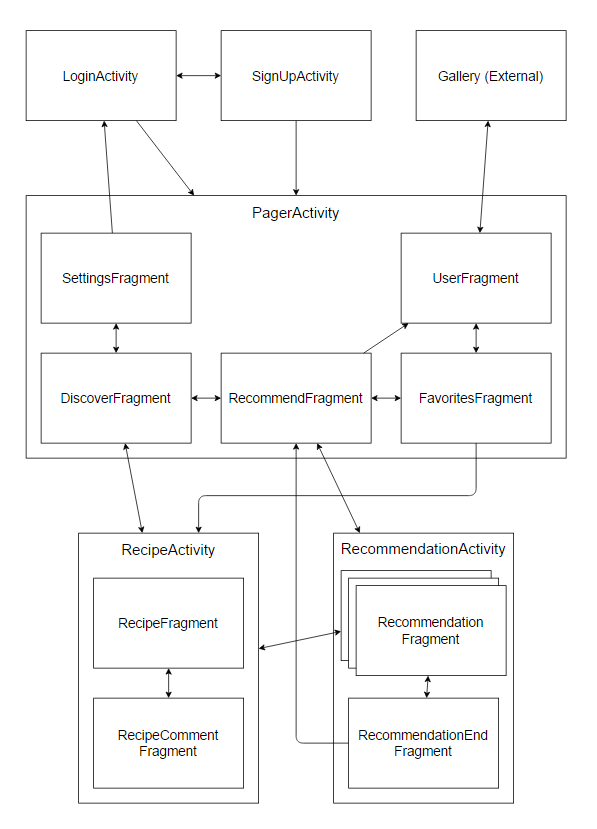
\includegraphics[width=\textwidth]{Pictures/application_navigation.png}
	\caption{Navigation paths in the application}
	\label{fig:application_navigation}
\end{figure}

\paragraph{Login- And SignUpActivity}
When launching the application, the \texttt{LoginActivity} is the point of entry. This obviously serves the purpose of logging the user into the application, but also enables the storage and retrieval of certain information under that particular user. Information about this can be seen in \todo{noget der ikke er skrevet endnu}. Furthermore, if the user has already logged in once, the \texttt{LoginActivity} is skipped entirely, launching the \texttt{PagerActivity} instead. This eases the use of the application, since users only have to login once. They will then stay logged in unless they manually log out.

For users who have not signed up yet, the \texttt{LoginActivity} features a link to the \texttt{SignUpActivity}. Through here, the user can create a new account. Besides from this, the functionality is similar to \texttt{LoginActivity}. Both screens feature a "Sign Up"/"Login" button, taking the user to the main user interface, the \texttt{PagerActivity}.

\paragraph{PagerActivity}
This \texttt{Activity} can be seen as the "Main Menu" of the application and features two elements. The first is the \texttt{ViewPager}. This is an Android component that allows \texttt{View} instances to be "paged". This allows the user to slide the views left or right, with another view coming into the screen. This can be read about at \citep{viewpager}.

This particular \texttt{ViewPager} holds five different \texttt{Fragment} instances. A \texttt{Fragment} is similar to an \texttt{Activity}. It has its own layout and lifecycle, but is possible to manipulate within a running \texttt{Activity}.\citep{fragment} For the purpose of this project, the fragments could have been an entire \texttt{Activity} each. But given the goal of making the GUI as fluent and simple as possible, using a \texttt{ViewPager} was a good way of eliminating excessive amounts of buttons and loading between five different \texttt{Activity} instances. \texttt{VievPager} does however use additional memory since it pre-loads the nearest fragments. For example, if \texttt{Fragment} 3 is currently shown to the user, \texttt{Fragment} 2 and 4 are also in memory, ready to slide onto the screen. This was however considered an acceptable trade-off.

The second element of the \texttt{PagerActivity} is a simple navigation bar, showing which window is currently shown, and letting the user press an icon to change the window. This exists for two reasons. One is to create a shortcut for the user. As worst example, going from the first \texttt{Fragment} to the last would require four swipes, which is now doable with one press. It is also to ensure that the user understands the navigation. Sliding on the screen is easy, but since only one \texttt{Fragment} is visible at a time, users can not know about the feature otherwise.

\paragraph{RecommendFragment}
The \texttt{RecommendFragment} is the what the user will encounter first upon logging in, or opening the application past the first login. The reason behind showing this exact fragment compared to one of the others, is that the application should be straight to the point. The application should be usable as a simple recipe application, but the recommendation feature is what distinguishies it, and what is hoped people will use it for.

The fragment consists of a single button that, when clicked, will find recommendations for the user. Assuming the user opened the application for ideas on what to make for dinner, it will always be just one click away. Furthermore, a link is provided to change recommendation preferences (\texttt{UserFragment}). This is to encourage that the user actively engages in what to weight in recommendations.

The fragment is placed in the middle of the \texttt{ViewPager}. In case a user did not launch the application to get a recommendation straight away, nothing is more than two swipes away (From \texttt{Fragment} 3 to 5 or 3 to 1).

\paragraph{UserFragment}
The \texttt{UserFragment} is where personal information is displayed. The user is able to change display name and profile picture. These informations are used when commenting on a recipe.
To enable profile pictures, the user will have to pick a photo from outside the application. This has been solved by launching a gallery application of the users choice, with the intent to choose a single picture. Upon doing so, the application is closed, and the path of the image returned to the \texttt{UserFragment} for display.

The \texttt{UserFragment} is also where recommendation preferences is changed. This is done with sliders, providing no details for the user. They should simply be arranged by importance. As such the user might see a preference for "Price", figure it is not very important and put the slider to a low value. These preferences will then affect the recommendations received when using the button in the \texttt{RecommendFragment}

\paragraph{FavoriteFragment}
Given that the application deal with finding good recipes it makes sense to have a \texttt{Fragment} that keeps track of the users favorite recipes. As such, this is where the user can go to find a list of favorite recipes. The recipes are shown by name and image, providing the option to remove them when long pressing a recipe. A normal press will open the recipe.

\paragraph{DiscoverFragment}
We recognize that users might not open the application for specific recommendations. This is where the \texttt{DiscoverFragment} comes into the picture. This \texttt{Fragment} is designed to be a recipe browser with a search feature. This helps when wanting something too specific for the recommender - for example recipes with chicken and bacon. Alternatively all recipes should be browsable by \todo{Hvad? Alfabetisk?}

\paragraph{SettingsFragment}
The last \texttt{Fragment} is for management on the application level. From here, the user can log out, which is not done upon closing the application. This enables the user to log in with another account if desired. One will also find preferences affecting both recommendations and recipes, such as the desired radius in which the application looks for prices on ingredients.

\paragraph{RecommendationActivity}
Upon clicking the button in the \texttt{RecommendFragment} in the \texttt{PagerActivity}, the user is taken to the \texttt{RecommendationActivity}, and more specifically a \texttt{RecommendationFragment}. The number of \texttt{RecommendationFragment} instances given stems from a user-defined setting and will as such vary. The \texttt{Fragment} instances consist of a presentation of a recommendation, along with two buttons. The buttons prompt the user to either choose the recipe (Opens the recipe), or move on to the next recommendation. In the case that the user does not want any of the recommended recipes, a final \texttt{Fragment} called \texttt{RecommendationEndFragment} will be shown, telling the user that there are no more recommendations to be seen. It also displays a button that closes the \texttt{RecommendationActivity}.

\paragraph{RecipeActivity}